%BEGIN JC
%\subsection{Isosurface Contouring}

In order to fit NURBS and other curves to an optimized geometry, a \emph{mesh-based geometry}, that is, a representation of the object at a set of (connected) points, is typically needed, this as opposed to the volumetric representation of density in each voxel, that results from the topology optimization process. 

In order to produce the mesh-based geometry, the data can be represented by a contour at a value of a smooth function in space, that is, an isosurface. Below, we describe two methods that solve this problem, the \emph{Marching Cubes} and the \emph{Dual Contouring} methods.% We then continue to discuss their applicability for NURBS curve fitting.

\subsection{Marching Cubes} 
%\subsection{Marching Cubes} 
\begin{figure}
\centering
   \scalebox{0.8}{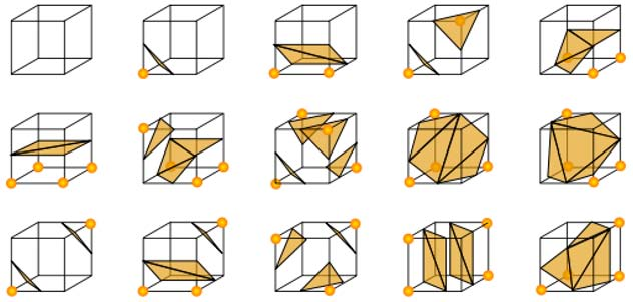
\includegraphics{Pictures/cubes.pdf}}\\
   \caption{The base cases of Marching Cubes. These are drawn with each polygon vertex intercepting its edge in the middle between the cube's corners, as in the case when the isovalue is exactly halfway between the function values at the vertices. Figure taken from \cite{Marching2006}. }
   \label{fig:MC_basecase}
\end{figure}
The Marching Cubes method \cite{Marching2006} takes as an input a set of scalar function values on a cartesian mesh and extracts an approximate isourface in the form of a mesh of triangles. The method starts by
dividing the space into cubes with the set of points as cube vertices. On these points, the value is determined to be above or below the desired isovalue. According to which corners are set to be above or below, the corner configuration is then mapped to a polygon inside the cube, with vertices on the cube's edges. On an edge between a vertex above and a vertex below the desired isovalue, the exact location of the surface is then determined via linear interpolation and set as the polygon's vertex on that edge.

%By connecting the vertices we obtain a polygon on each cube. 
Since there are 8 vertices on each cube, each above or below the isovalue (with equality falling to one of these categories), there are $2^8=256$ possible polygon configurations. However, many of these can be constructed by rotating or reflecting other polygons. As such, there are therefore 15 base cases which represent all the surface polygons of the marching cubes. To illustrate what the polygons may look like, these are shown in \autoref{fig:MC_basecase}, where one can also see that they are composed of triangles. 
The original algorithm presents two main problems. Firstly, it does not guarantee neither
correctness nor topological consistency, which means that holes may appear on the surface due
to inaccurate base case selection. Second, another problem is ambiguity, which appears when two
base cases are possible and the algorithm chooses the incorrect one. There are many extended Marching Cubes
algorithms that tackle the problems of the original one, getting rid of the ambiguities and
providing correctness (see for example \cite{ExtendedMC}).

%\subsection{Dual Contouring}
\subsection{Dual Contouring}
The idea of \emph{Dual algorithms}, to which Dual contouring belongs, is similar to Marching Cubes. However, instead of generating polygon vertices on the
edges of the cubes, it locates them inside the cubes that have vertex values both above and below the isovalues.
After locating the vertices, the ones associated with four contiguous cubes are joined to form a quadrilateral face, commonly referred to as a \emph{quad}. The approach can be seen in \autoref{fig:bunny_MCDC}, with a similar Marching Cubes illustration for comparison. 

The relevant question is now where in the cube the ideal place for the vertex is, and here is where different dual algorithms are distinguished. Dual Contouring in particular generates a vertex positioned at the minimizer of a
certain quadratic function, which depends on the (interpolated) isosurface intersection points, as well as the gradient -- or just the normal of the isosurface -- at these points, together the first-order \emph{Hermite data} of the set.
The quadratic function for Dual Contouring is defined in \cite{Hermite2002} as follows:
\begin{equation*}
E(x)= x^TA^TAx-2x^TA^Tb+b^Tb
\end{equation*}
where \textit{A} is a matrix whose rows are the isosurface normals at the intersection points, and \textit{b} is a vector whose entries are the product of normals and the intersection points. This system can be solved numerically, for example as proposed in \cite{Hermite2002} by computing the
singular value decomposition of \textit{A} and forming the pseudo-inverse, truncating its small singular values. 
%1=Dual Contouring of HErmite DAta


The main advantage of this method over Marching Cubes is the acquisition of better aspect ratios \cite{Hermite2002}. On the other hand the need of gradient data
represents a disadvantage. %Furthermore, there is no open source algorithm that implements the Dual Contouring scheme. %well, it says later on VTK has one...



%\subsection{VTK Toolbox}
%\subsubsection{Installing VTK}
%VTK was installed using the Linux platform with pre-installed gcc. VTK offers the possibility to use Python, TLC or C++ for
%development. VTK toolbox is actually a C++ library, which is implemented in other languages. We
%decided to continue the project with C++ since it gives the possibility to explore the original code.
%%A few dependency problems were encountered, nevertheless they were easy to track back. If any
%problems were to be found at installation time, please refer to the VTK Wiki where the procedure
%is explained step by step.


%\subsubsection{Implementing the VTK Classes}
%\subsection{VTK Toolbox}
\begin{figure}
\centering
   \scalebox{0.35}{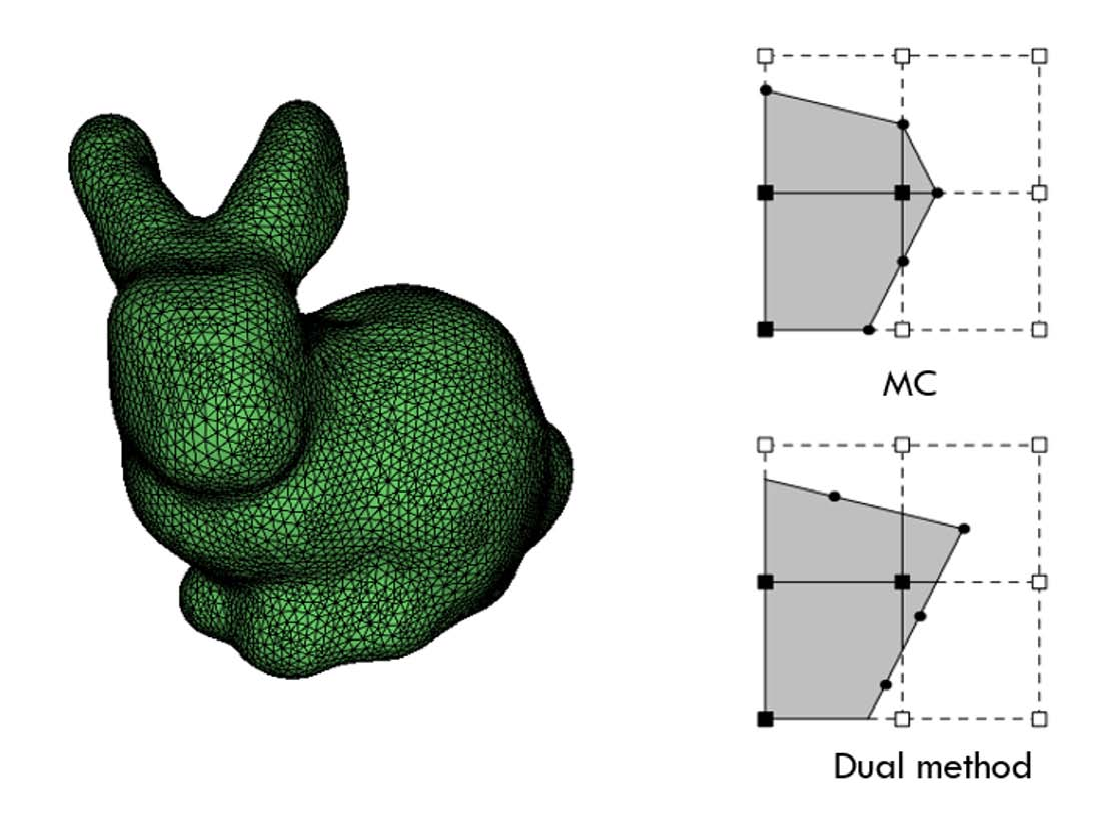
\includegraphics{Pictures/bunny_MC.pdf}}\\
   \caption{\textit{Left:} The famous Stanford Bunny, a popular computer graphics test object, here after application of Marching Cubes. \textit{Right:} Main difference between MC and Dual methods.  Figures taken from \cite{Hermite2002}. }
   \label{fig:bunny_MCDC}
\end{figure}
%The VTK toolbox was used in order to implement the algorithms on our optimized data. It is a heavily object
%oriented toolbox. Our first approach was to use the built in Marching Cubes algorithm,
%nevertheless it did not work with our unstructured grid data. It just works for ImageData and
%PolyData . For structured and unstructured grids the tool to render the isosurface is the \textit{Contour Filter} tool. Unfortunately the documentation does not present which algorithm the tool uses. It
%can be inferred that it is an extended Marching cubes algorithm.



%It finally allowed visualization but it created one problem. Holes are lost in
%the process.




%%%%%% THIS PART WILL BE INCLUDED IN THE NEXT M. in case this approach is needed.

%\subsection{Voxel Data to NURBS}
%There are two possible roads to go from the voxel data to the CAD representation (in our case NURBS based representation).
%\subsubsection{Quad Contouring}
%This approach uses the Dual Contouring algorithm as first step in order to obtain a quad mesh
%representation from the voxel data. The first challenge is to implement the algorithm
%with the ideas presented in \cite{Hermite2002} correctly. The original Marching Cubes algorithm is
%implemented in VTK but the source code is not public. Once this first step is done, the quads will be chosen for the
%NURBS parametrization. A second step considers multiple smaller quads which have to be
%combined into one larger patch. This is another challenge, since the remeshing of quad meshes
%is not as straightforward as with the triangles. Different approaches have been taken in order to achieve this coarsening. In \cite{Puppo2010} an incremental and greedy approach, which is based on local operations only, is presented. It depicts an iterative process which performs local optimizing, coarsening and smoothing operations. Other approaches, like the one presented in \cite{Dong2005} uses smooth harmonic scalar fields to simplify the mesh.

%2= “Practical quad mesh simplification”
%3= “Harmonic Functions for Quadrilateral Remeshing of Arbitrary Manifolds”


%\subsubsection{Multiresolution Analysis of Arbitrary Meshes}
%With \textit{Multiresolution Analysis of Arbitrary Meshes} approach there is no need to apply a Dual Contouring algorithm, since it takes as
%beginning data the triangles from the Marching Cubes. The main concepts are shown in the paper \cite{eck1996automatic}. It mainly takes a series of intermediate steps which permits a parametrization of data. It includes a partitioning scheme based on the ideas of the Voronoi Diagrams %reference
 %Delaunay triangulations %reference
. %Large patches or quads are obtained with this method. 

%4=reference to MAAM, a.k.a Benni's favorite paper!

%%implementation part!
%Both approaches have not been implemented in open source documentation, therefore there is a need to implement it from scratch. Up to now, the second approach has been chosen.

%END JC
